\documentclass[10pt,a4paper]{labreport}
\usepackage{csquotes}
\usepackage{titlesec}
\usepackage{ragged2e}
\usepackage{siunitx}
\AtBeginDocument{\RenewCommandCopy\qty\SI}
\usepackage{setspace}
\usepackage{longtable}
\usepackage{rotating}
\usepackage{xurl}
\usepackage{physics}
\usepackage{caption}
\usepackage{wrapfig}
\usepackage{tabularray}
\usepackage{fancyhdr}
\usepackage{subcaption}
\usepackage{lscape}
\usepackage{tensor}
\usepackage{multirow}
\usepackage[gen]{eurosym}
\usepackage{float}
\usepackage{bm}
\usepackage{lipsum}
\usepackage{parskip}
\usepackage{booktabs}
\usepackage{enumerate}
\usepackage{needspace}
\usepackage[justification=justified]{caption}
\usepackage[nottoc]{tocbibind}
\usepackage{hyperref}
   \usepackage[
  backend=biber,
  style=chem-acs,articletitle=true,doi=true]{biblatex}
  \addbibresource{references.bib}
\usepackage{color}

\usepackage{listings}
\definecolor{codegreen}{rgb}{0,0.6,0}
\definecolor{codegray}{rgb}{0.5,0.5,0.5}
\definecolor{codepurple}{rgb}{0.58,0,0.82}
\definecolor{backcolour}{rgb}{0.95,0.95,0.92}
\lstdefinestyle{mystyle}{
    backgroundcolor=\color{backcolour},   
    commentstyle=\color{codegreen},
    keywordstyle=\color{codepurple},
    numberstyle=\tiny\color{codegray},
   % stringstyle=\color{grey},
    basicstyle=\ttfamily\footnotesize,
    breakatwhitespace=false,         
    breaklines=true,                 
    captionpos=b,                    
    keepspaces=true,                 
    numbers=left,                    
    numbersep=5pt,                  
    showspaces=false,                
    showstringspaces=false,
    showtabs=false,                  
    tabsize=5
}
\lstset{style=mystyle}




\title{Nanoscale Material Modeling
\\
\normalsize{Week 7}} % Main title and sub title. 

\author{Ilija A. Gjerapić, S4437586; \href{mailto:i.a.gjerapic@student.rug.nl}{i.a.gjerapic@student.rug.nl}; \href{https://github.com/igjerapic/nmm-week7/}{@github} } % Name, student number, email

\supervisors{prof. dr. A. Giuntoli, prof. dr. J. Slawinska}

\begin{document}


\maketitle
\tableofcontents


  

\thispagestyle{firststyle}
\newpage
\section{Assignment 1: Back to Silicon}

\subsection{Simulation workflow}
The simulation iteratively calculates through the columns of the 6$\times$6 elastic tensor by performing a small deformation in the $u_{xx},u_{yy},u_{zz},u_{yz},u_{xz}, u_{xy}$ directions. 
Before any deformation, the silicon crystal is equilibrated.  

The calculation of the  elastic tensor columns is completed using the following algorithm along the previously mentioned directions:
\begin{enumerate}
  \item Set conditions to probed equilibrated state
  \item Perform negative deformation (compression)
  \item Calculate elastic constant from the change in the respective component of the pressor tensor e.g.
  $$ C_{11} = -\frac{p_{xx} - p_{xx,0}}{\delta},$$
  where $\delta$ is the displacement, and $p_{xx}$ the new component of the pressure tensor and $p_{xx,0}$ the original component of the pressure tensor.  
  \item Revert to probed equilibrated state
  \item Perform a positive deformation (elongation)
  \item Calculate elastic constant from the change in the respective component of the pressor tensor similar as in step 2.
  \item The final elastic constants of the column are taken as the average between the value calculated for the positive and negative deformation. 
  \item Repeat for the remaining directions to obtain full elastic tensor. 
\end{enumerate} 
As the elasticity tensor is symmetric, the off-diagonal elements of the final elasticity tensor are taken as the average between the two corresponding off-diagonal elements of the elasticity tensor calculated using the above algorithm.   

For an interaction strength of 2.1683 eV, the final elasticity tensor in GPa is:
\begin{equation}
  C_{ij} = \left[
  \begin{array}{llllll}
         151.4        &      76.42        &      76.42        & -4.032\text{e-}08 & -7.779\text{e-}08 &  8.662\text{e-}09 \\ 
     76.42            &      151.4        &      76.42        &  5.804\text{e-}08 & -6.665\text{e-}08 &  2.349\text{e-}08 \\ 
     76.42            &      76.42        &      151.4        &  1.933\text{e-}08 & -7.822\text{e-}09 & -9.292\text{e-}09 \\ 
-4.032\text{e-}08     &  5.804\text{e-}08 &  1.933\text{e-}08 &      56.45        &  1.491\text{e-}07 &  1.078\text{e-}08 \\ 
-7.779\text{e-}08     & -6.665\text{e-}08 & -7.822\text{e-}09 &  1.491\text{e-}07 &      56.45        & -4.517\text{e-}08 \\ 
 8.662\text{e-}09     &  2.349\text{e-}08 & -9.292\text{e-}09 &  1.078\text{e-}08 & -4.517\text{e-}08 &      56.45 
  \end{array}
   \right],
   \label{eq:ass1_elasticity_final}
\end{equation}
where $i,j \in \{xx, yy, zz, yz, xz, xy\}$. This elasticity tensor corresponds the average material properties for a cubic crystal shown in Table \ref{tab:ass1_mechprops}.
\begin{table}[h]
  \centering
  \caption{The average mechanical properties for a cubic crystal as derived from the elasticity tensor in equation \eqref{eq:ass1_elasticity_final}. For comparison, the analytical values for the  Stillinger-Weber model of silicon and experimental values from reference \cite{cowleyLatticeDynamicsSilicon1988} are included. }
  \begin{tabular}{ccccc } \hline 
    Property & Bulk Modulus (GPa ) & Shear Modulus 1 (GPa) & Shear Modulus 2 (GPa) & Poisson Ratio \\ \hline
    Computed & 101.42 & 56.45 & 37.5 & 0.34 \\
    Analytical & 101.4 & 56.4 & 37.5 & 0.34 \\ 
    Experiment & 97.83 & 79.6 & 50.9 & 0.29 \\
    \hline 
  \end{tabular}
  \label{tab:ass1_mechprops}
\end{table}

\newpage
\subsection{Enthalpic Nature}
To investigate the enthalpic nature of elasticity, the interaction energy was varied from 1.0 eV to 4.5 eV in steps of 0.5 eV. 
The dependence of the bulk elastic modulus on the interaction energy is shown in Figure \ref{fig:ass1_moduli-vs-epsilon}. The elastic modulus increases linearly with the interaction energy, showcasing the enthalpic nature of elasticity.
\begin{figure}[h]
  \centering
  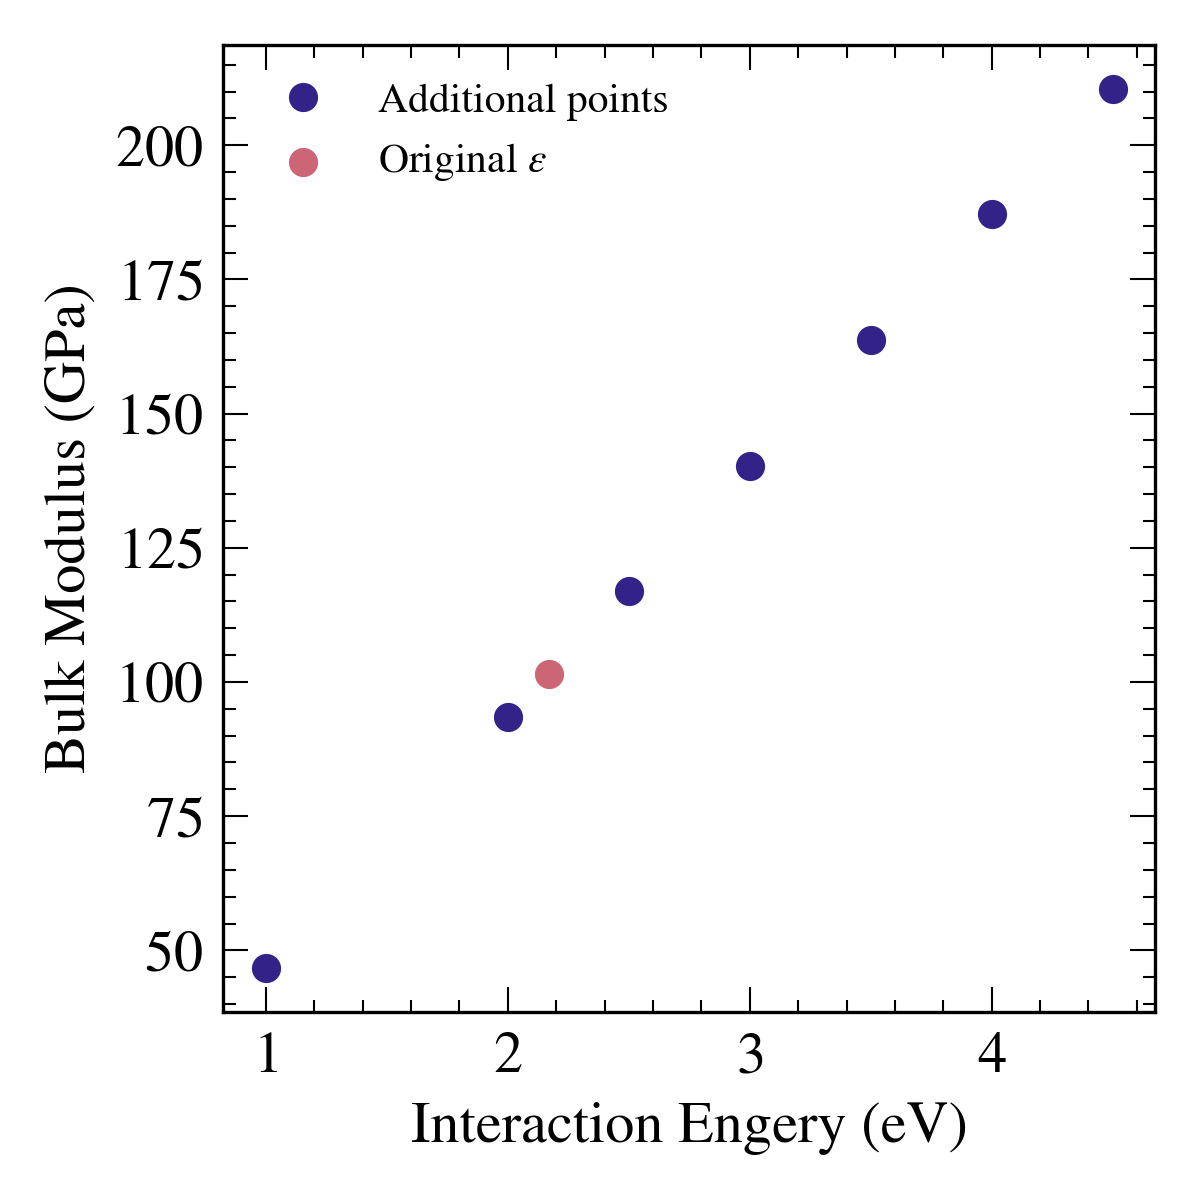
\includegraphics[width = 0.6\textwidth]{figs/ass1_moduli-vs-epsilon.png}
  \caption{The bulk modulus for a cubic crystal of silicon as a function of increasing interaction energy. The elastic modulus increases linearly with the interaction energy, showcasing the enthalpic nature of elasticity.}
  \label{fig:ass1_moduli-vs-epsilon}
\end{figure}

\newpage
\section{Assignment 2: Not everything is a spring}
\subsection{Fraction Simulation}
\subsubsection{Simulation Protocol}
The simulation includes a slab of silicon with dimensions of 20x20x10 diamond lattices with lattice constant 5.43 \AA. The simulation has shrink-wrapped boundaries in x,y directions and a periodic boundary in the z-direction. 
To enforce the notch deformation, the slab is split into five different sections as shown in Figure \ref{fig:ass2_crack-setup}. 
\begin{figure}[h]
  \centering
  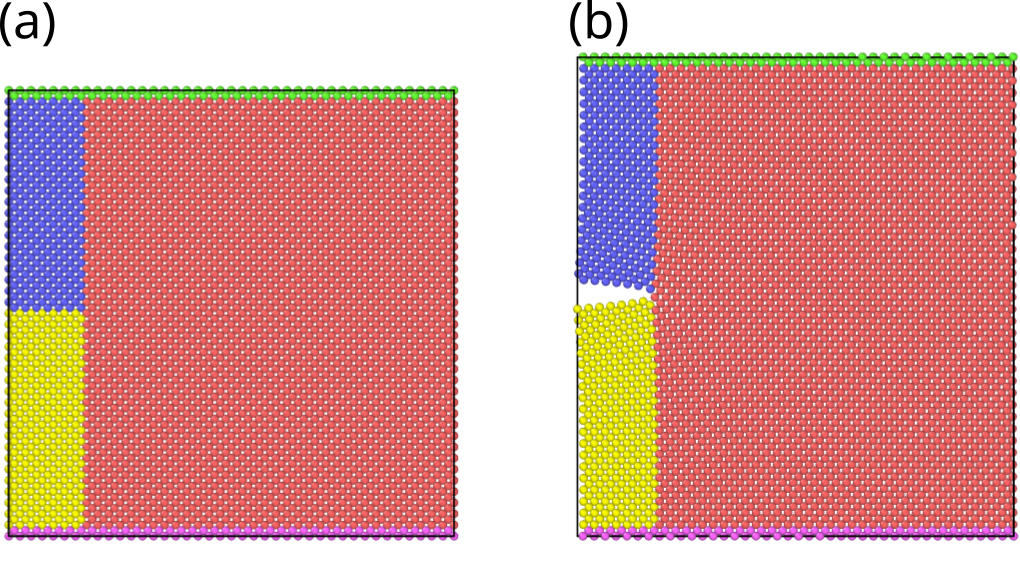
\includegraphics[width=0.75\textwidth]{figs/ass2_crack_setup.png}
  \caption{The simulation setup used to enforce the notch deformation. The notch was formed by excluding pair-wise interactions between the blue and yellow atoms. The deformation was induced by fixing the velocity of the green atoms to a set value in the y (up) direction and fixing the y-component of the force on the green and purple atoms to be zero. No extra constraints were enforced on the red atoms. The width of the region containing red atoms is 18.1 \AA. (a) Shows the simulation at time $t=0$ps while (b) shows the notch formation after several time steps. }
  \label{fig:ass2_crack-setup}
\end{figure}

The notch is formed by excluding interactions between the upperleft (blue) and lowerright (yellow) atoms using the \texttt{neigh\_modify} command with the \texttt{exclude} keyword, see Listing \ref{lst:notch_exclude}.

\begin{lstlisting}[
                  caption={The LAMMPS command to generate the notch between the blue and yellow group of atoms shown in Figure \ref{fig:ass2_crack-setup}. The command tells LAMMPS to ignore pair-wise interactions between atoms of type 2 (blue atoms) and type 3 (yellow atoms). Other than this, the atoms have no other special conditions.},
                  label=lst:notch_exclude,
                  ]
neigh_modify exclude type 2 3 # type 2 are blue atoms type 3 are yellow atoms
\end{lstlisting}

The deformation is enforced by the fixing the force in the y-direction of of the bottom (purple) and top (green) to zero. Moreover, the top (green) atoms have a fixed velocity in the y-direction, This is enforced using the commands shown in Listing \ref{lst:notch_deform}. The red atoms have no special conditions. 
\begin{lstlisting}[
                  caption={The LAMMPS command to initite deformation of the silicon slab. The upper group consists of the green atoms in Figure \ref{fig:ass2_crack-setup}. The boundary group includes both the green and purple atoms in Figure \ref{fig:ass2_crack-setup}.},
                  label=lst:notch_deform,
                  ]
velocity upper set 0.0 0.5 0.0          # 0.5 velocity in y-direction
fix  2 boundary setforce NULL 0.0 NULL  # enforce no y-component force
\end{lstlisting}


\subsection{Different pulling rates}
The velocity of the top atoms is here called the pulling rate and was simulated at 0.2,0.5, and 0.75 \AA/ps. 
The effect of pulling speed on the crack the fracture was investigated by visually determining  when the crack started to propagate and when the fracture propagated approximately 18.1\AA (the entire red region of Figure \ref{fig:ass2_crack-setup}). 

The fracture behavior was quantified by considering the displacement of the upper layer $\delta$ at the start of the crack propagation, the total time $\Delta t$ of the crack propagation, and the propagation speed $v$ of the fracture.   
The results of the visual analysis are summarized in Table \ref{tab:ass2_film_props}. 
Figure \ref{fig:ass2_cracks} shows \texttt{ovito} snapshots of the frames that were considered for the visual analysis. 
\begin{table}
  \centering
  \caption{The displacement $\bm{\delta}$ of the upper atoms  at which the crack propagation starts, the propagation time $\bm{\Delta t}$ of the crack, and the corresponding speed $\bm{v}$ resulting from the visual analysis for different pull rates. The uncertainty of each value stems from the uncertainty in determination of the time at which the crack propagation started and ended. This was arbitrarily set to be two frames, corresponding to 0.1 ps. }
  \begin{tabular}{cccc} \hline \\[-0.8em]
    \textbf{Pull Rate \AA/ps} & \textbf{$\bm{\delta}$ \AA}  & \textbf{$\bm{\Delta t}$ ps $\pm$ 0.2 ps} & \textbf{$\bm{v}$ \AA/ps} \\ \hline
    0.2  & $2.37 \pm 0.02$ & 1.5 & $12.1 \pm 0.8$ \\
    0.5  & $2.40 \pm 0.05$ & 1.0 & $18 \pm 2$ \\
    0.75 & $2.40 \pm 0.08$ & 0.9 & $20 \pm 2$ \\ \hline 
  \end{tabular}
  \label{tab:ass2_crack-props}
\end{table}
The crack started to propagate at approximately the same upper region displacement of 2.4 \AA. 
The speed of the fracture propagation was found to range from ($12.1 \pm 0.8$) \AA/ps to $(20 \pm 2)$ \AA/ps.  
These values are reasonably close to reported literature values of 15\AA/ps to 35 \AA/ps \cite{rackRealtimeDirectDiffraction2016}. It seems as if the behavior of the fracture, once it begins is independent of the pull rate. This is likely due to the crack propagation speed being several orders of magnitude larger than the pulling rates investigated. 
\begin{figure}[h]
  \centering
  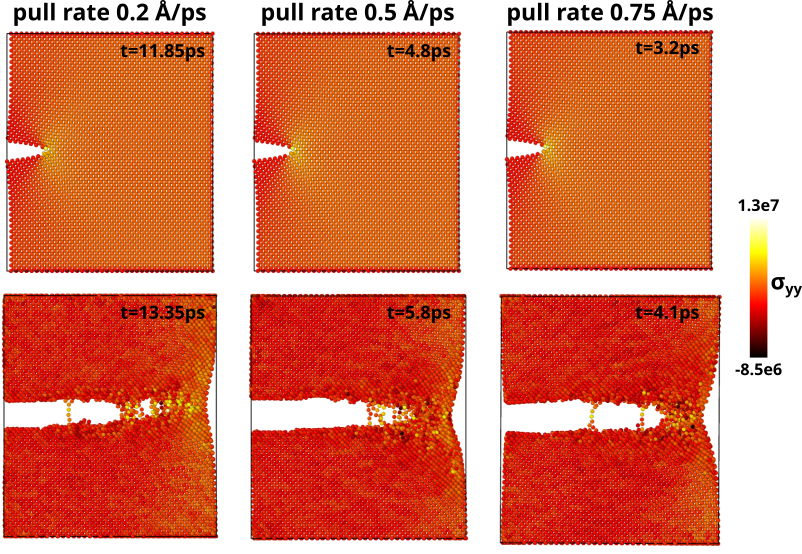
\includegraphics[width = \textwidth]{figs/ass2_cracks.png}
  \caption{The visualizations used for the characterization of the crack propagation. The top row demonstrates the start of the crack propagation while the bottom row shows what was considered to be the end of the crack propagation. The atoms in each image are colored according the YY stress component. }
  \label{fig:ass2_cracks}
\end{figure}

\newpage
\subsection{Polymer Films}
A bead-spring model with harmonic bonds and LJ non-bonded interactions is used for the polymer chains in all three films. For direct neighbors, only bonded interactions are considered. 
\begin{align}
  E_\text{bond} = K (r - r_0)^2;&~~ K=2500,~r_0 = 0.9 \\
  E_\text{LJ} = 4\epsilon\left[\left(\frac{\sigma}{r}\right)^{12} - \left(\frac{\sigma}{r}\right)^6\right], r < r_c ;& ~~ \epsilon = 1.0, ~\sigma = 1.0, ~ r_c = 2.5
\end{align} 
The difference between the three polymer films is the chain length, with film 1,2,3 consisting of polymers with length 10, 20, and 50, respectively.

The strain-stress curves along with \texttt{ovito} visualizations of each film deformation are shown in Figure \ref{fig:ass2_deform_films}. 
To quantify the strain response of each film, the maximum stress, elongation, and fracture energy were considered \cite{zhangUnderstandingCavitationCrazing2020}. 
The elongation was considered as the strain at which the stress becomes zero again, within a tolerance of 0.01. 
The fracture energy is taken as the area under the stress-strain curve. 
Table \ref{tab:ass2_film_props} summarizes these properties for each film. 
\begin{table}[h]
  \centering
  \caption{The quantitative values of the stress-strain curves for the three films considered. The elongation is considered as the first zero-stress strain after the maximum stress within a tolerance of 0.01. The fracture energy is the area under the stress-strain curve \cite{zhangUnderstandingCavitationCrazing2020}.}
  \begin{tabular}{cccc}
    \hline
    \textbf{Film} & \textbf{Max Stress} & \textbf{Elongation} & \textbf{Fracture Energy} \\ \hline
    1 & 2.12 & 0.56 & 0.71 \\
    2 & 2.19 & 0.86 & 1.22 \\
    3 & 2.24 & 1.41 & 1.29 \\
    \hline
  \end{tabular}
  \label{tab:ass2_film_props}
\end{table}

Each stress-strain curve has the same elastic deformation region with approximately the same maximum stress point. 
However, the films with  longer chains are able to experience larger strains without failure. 
This is attributed to the ability of longer chains to dissipate energy through chain extension which leads to crazing rather than fracture.  
\begin{figure}[p]
  \centering
  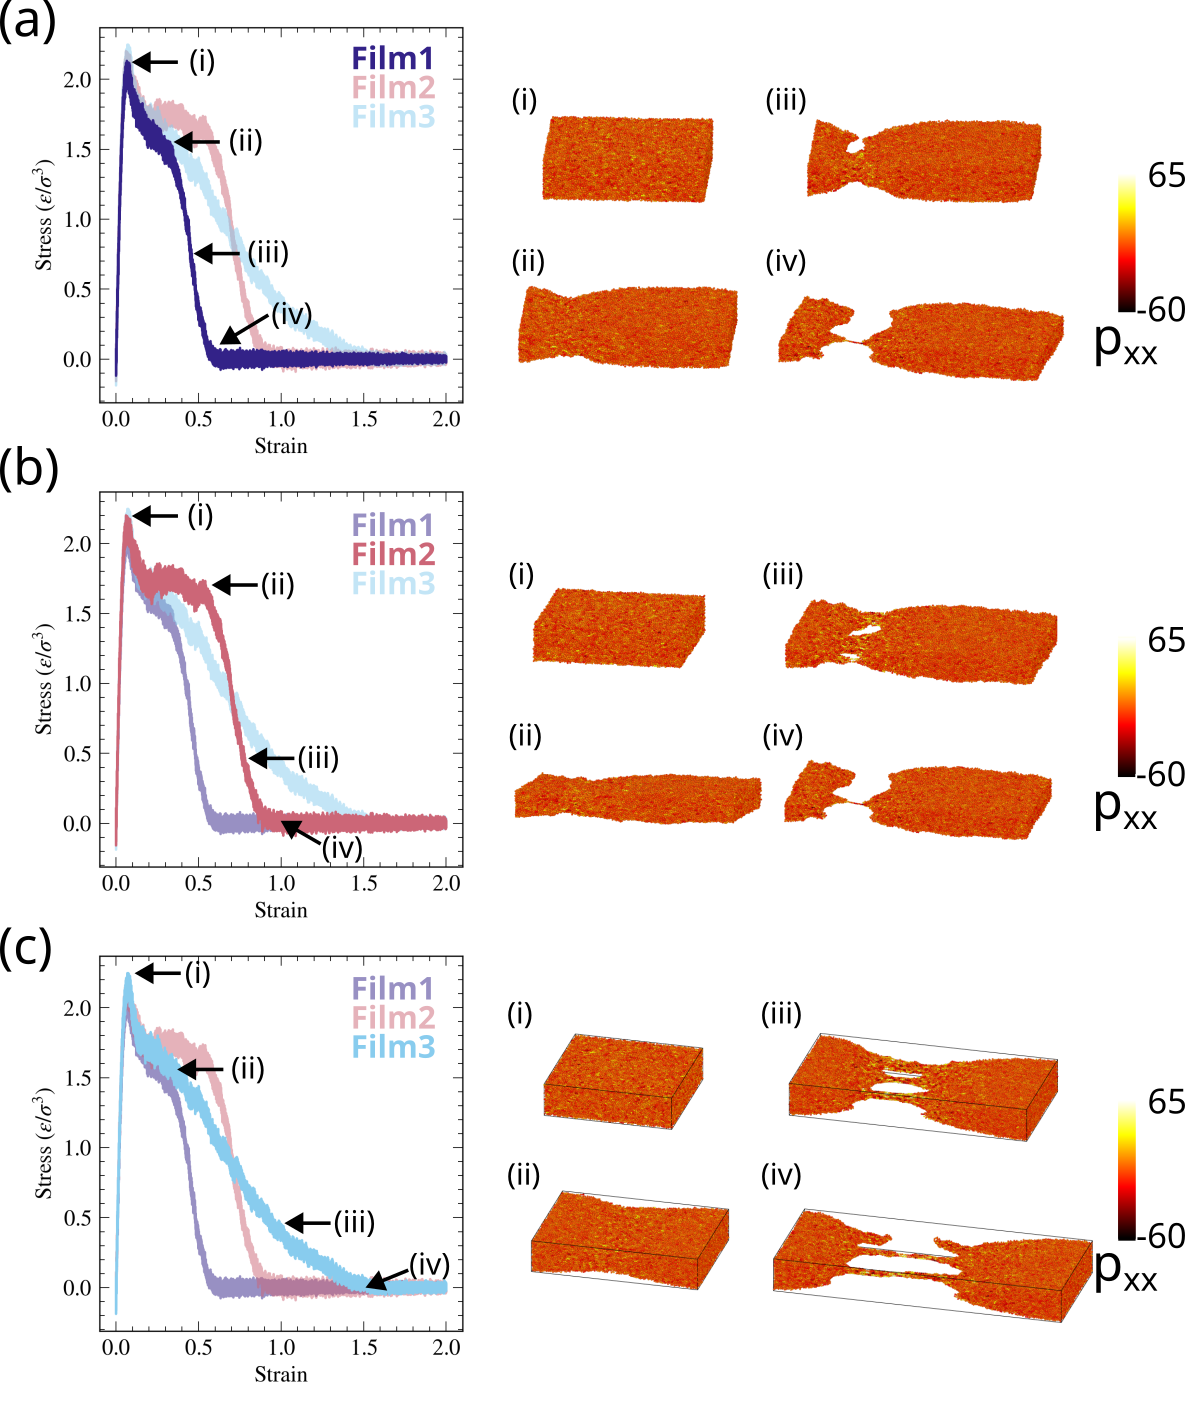
\includegraphics[width= \textwidth]{figs/ass2_films_results.png}
  \caption{The stress-strain curves (left) and \texttt{ovito} snapshots corresponding to the annotations  colored by the stress/atom (right) for (a) film 1 (b) film 2 (c) film 3. The stress-strain curves for the other films are shown in opaque colors for easier comparison. Annotated points include (i) the maximum stress point, (ii) the start of elongation/claving and the end of plastic deformation (iii) a point during claving and (iv) the elongation point. Films with longer chains show longer elongation due to the ability to dissipate energy through chain extension. }
  \label{fig:ass2_deform_films}
\end{figure}


\newpage
\section{Assignment 3: Bound to Succeed}
The filler particle is modelled as a sphere of 625 beads whose positions are tethered to their initial positions with a spring constant of 1000. 
This allows for the ability to tune the hardness of the filler particle.
The filler particle is surrounded by 999 polymers of length 50 which are modelled as bead-springs with a FENE potential. 
The size of the filler particle beads is the same as the beads of the polymers.
The interaction energy between the filler particle and the polymers is set to 5.0 while inter-particle interactions have an energy of 1.0.  
An \texttt{ovito} visualization of the system is shown in Figure \ref{fig:ass3_struct}(a). The summary of the structural and dynamics length-scales of the bound layer is shown in Table \ref{tab:ass3_length_scales}.

\begin{table}[h!]
  \centering
  \caption{The structural and dynamics length scale in $\bm{\sigma}$ of the bound layer of polymers on the filler particle surface. The structural length scale was determined from particle density, while the dynamics from the Debye-Waller factor. }
  \begin{tabular}{cc}
    \hline
    \textbf{Structural} & \textbf{Dynamics} \\ \hline
    2.58 & 2.975  \\ \hline
  \end{tabular}
  \label{tab:ass3_length_scales}
\end{table}

\subsection{Structural Analysis}
The radial polymer bead density around the center of mass of the filler particle is shown in Figure \ref{fig:ass3_struct}(b). The density is initially zero for distances up to approximately 5.0 $\sigma$, which is attributed to the radius of the filler particle. After 5.0 $\sigma$, there is a series of large peaks which decay to a constant value after a distance of 10.0 $\sigma$. The peaks are related to a dense layer of polymers that are bound to the surface of the nanoparticle, while the plateau value is the density of the bulk polymer melt. The structural length scale of the  bound layer is quantified by taking the distance of the first peak that is below 34\% of the maximum density peak. This provides a structural length-scale of 2.58 $\sigma$. 
\begin{figure}[h]
  \centering
  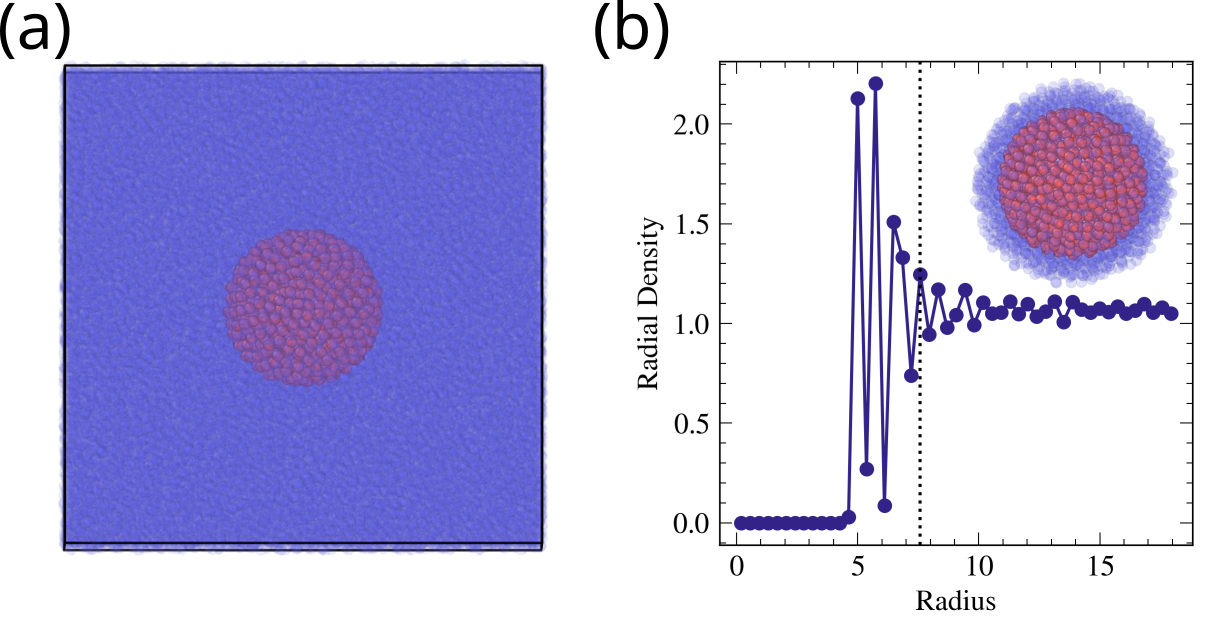
\includegraphics[width = 0.75\textwidth]{figs/ass3_struct.png}
  \caption{(a) An \texttt{ovito} visualization of the filler particle (red) surrounded by bead-spring polymers of length 50 (blue). The polymers have been shown with increased transparency for clarity. (b) The bead density of spherical shells around the filler particle as function of the radial distance from the COM of the particle. The initial zero values are attributed size of the filler particle. The strong peaks after 5 $\sigma$ are considered to be the bound layer, while the plateau value is the bulk density. The bound layer (black dotted line) is determined by the first peak less than 34\% of the maximum peak. A structural length scale of 2.58 $\sigma$ is determined. The inset shows an \texttt{ovito} visualization of the filler particle with the boundary layer corresponding to this length-scale. }
  \label{fig:ass3_struct}
\end{figure}

\subsection{Dynamical Analysis}
The dynamics of the bound layer was considered by investigating the MSD and Debye-Waller factor (DWF) for nine concentric spherical shells of thickness 1.35 $\sigma$ around the filler particle. The MSD and DWF for the shells are shown in Figure \ref{fig:ass3_dynamics}(a) and Figure \ref{fig:ass3_dynamics}(b), respectively.

The MSDs of the different shells first show a sharp increase up to about 0.1 $\tau$, followed by a plateau, and ends with an increase for shells 2-9.
The initial increase in the MSD is due to the beads exploring their local neighborhood.
The plateau in the MSD is indicative of kinetically frustrated beads.
The final increase in MSD for shells of larger radii indicates the diffusion of the beads from their kinetically trapped state.  
The MSD shows that the polymer beads closer to the surface of the filler particle experience slower dynamics.  

The dynamics of the polymer as a function of the distance to the filler particle surface can be probed further by considering the Debye-Waller factor, $\langle u^2 \rangle = MSD(\tau = 1.0)$. 
The Debye-Waller factor quantifies the average amplitude of the polymer beads motion rising from thermal fluctuations at the time scale of caging (during the plateau of the MSD) \cite{zhuEffectNanoparticleSoftness2022a}.  
The Debye-Waller factor shows a sharp increase, followed by a plateau, showing the slower dynamics at the interface.

The dynamics length scale is determined by taking the first distance at which the DWF is larger than the 64\% of the average plateau values. 
This leads to a dynamics length-scale of 2.975 $\sigma$.  

\begin{figure}[h]
  \centering
  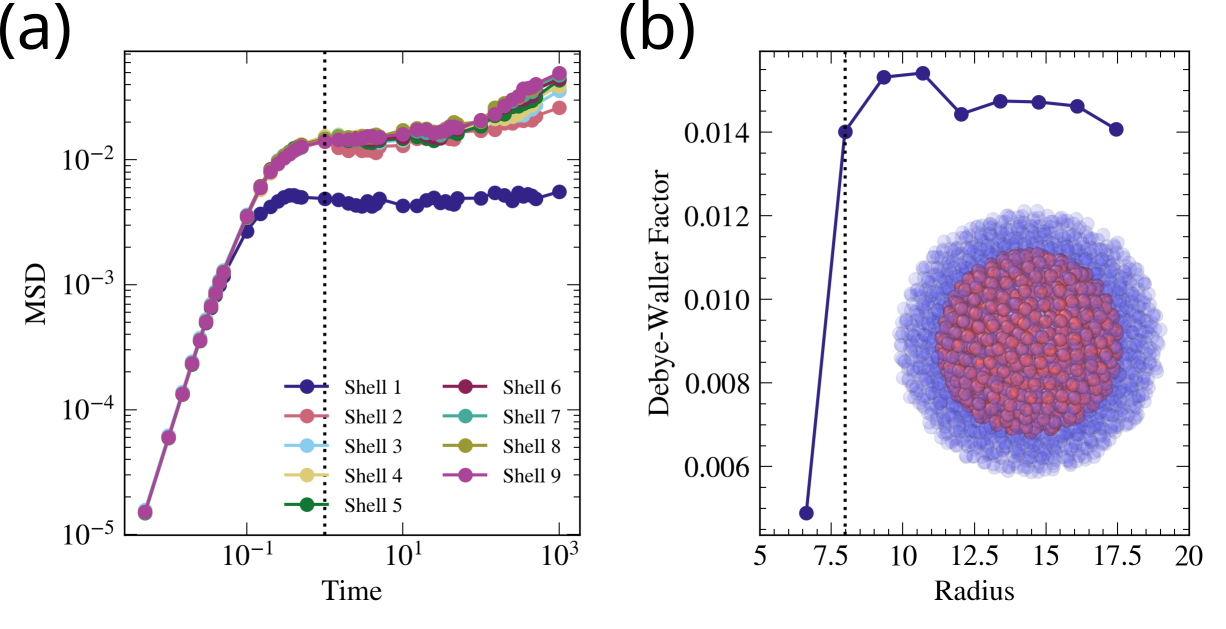
\includegraphics[width = 0.75\textwidth]{figs/ass3_dynamics.png}
  \caption{(a) The MSD averaged for polymer beads in different concentric spherical shells of thickness 1.35 $\sigma$. Each shell demonstrates caging dynamics from the plateau in the MSD. Particles further from the filler particle surface show additional diffusive behavior after around 10$^2~\tau$. The black dotted line shows $Time = 1.0 \tau$ from which the Debye-Waller factor was determined. (b) The Debye-Waller factor of each shell as a function of the distance from the COM of the filler particle. The distance was taken as the middle radius of the spherical shell. Slower dynamics are observed closer to filler particle with a plateau of faster dynamics for further distances (bulk melt). A dynamics length scale of 2.975 $\sigma$ (black dotted line) was determined by taking the first distance with a DWF greater than 64\% of the plateau. The inset shows an \texttt{ovito} visualization of the filler particle with the boundary layer corresponding to this length-scale.  }
  \label{fig:ass3_dynamics}
\end{figure}

\printbibliography

% \begin{appendices}
%   \input{Appendix}
% \end{appendices}

\end{document}



